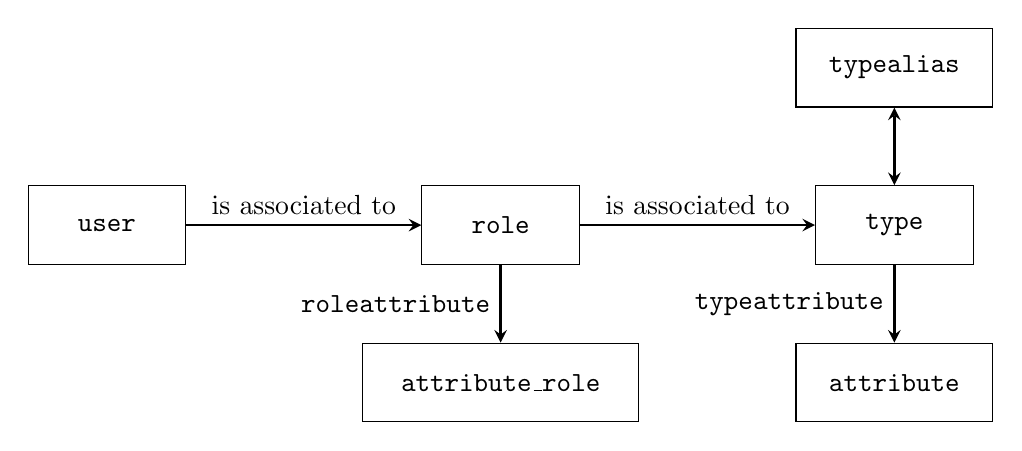
\begin{tikzpicture}
    \usetikzlibrary{calc}
    \tikzstyle{arrow} = [->,>=stealth, line width=1pt]
    \tikzstyle{darrow} = [<->,>=stealth, line width=1pt]
    \tikzstyle{rec} = [rectangle, draw=black, align=center, text width=3.5cm,
        minimum height=1cm, minimum width=4cm, fill=white]

    \node(user) [rec, text width=1.5cm, minimum width=2cm]
        at (0,-0.5) [anchor=north west]
        {\textbf{\texttt{user}}};

    \node(role) [rec, text width=1.5cm, minimum width=2cm]
        at (5,-0.5) [anchor=north west]
        {\textbf{\texttt{role}}};

    \node(type) [rec, text width=1.5cm, minimum width=2cm]
        at (10,-0.5) [anchor=north west]
        {\textbf{\texttt{type}}};

    \node(roleattr) [rec, text width=3cm, minimum width=3.5cm]
        at (4.25,-2.5) [anchor=north west]
        {\textbf{\texttt{attribute\_role}}};

    \node(typeattr) [rec, text width=2cm, minimum width=2.5cm]
        at (9.75,-2.5) [anchor=north west]
        {\textbf{\texttt{attribute}}};

    \node(typealias) [rec, text width=2cm, minimum width=2.5cm]
        at (9.75,1.5) [anchor=north west]
        {\textbf{\texttt{typealias}}};

    \draw[arrow] (user) -- node[pos=0.5,above] {is associated to} (role);
    \draw[arrow] (role) -- node[pos=0.5,above] {is associated to} (type);
    \draw[darrow] (typealias) -- (type);
    \draw[arrow] (role) -- node[pos=0.5,left] {\texttt{roleattribute}}
        (roleattr);
    \draw[arrow] (type) -- node[pos=0.5,left] {\texttt{typeattribute}}
        (typeattr);
\end{tikzpicture}
